\chapter{はじめに}
被災地での救助活動を行う際に,訓練されたレスキュー犬(災害救助犬)が人間の補助として探査を行う場合がある~図\ref{resque}.災害救助犬を育成し、現場に派遣する団体は日本国内に複数存在し
、必要に応じて現場に派遣される。
レスキュー犬は,犬としての特性を生かして人間と協力して被災地の探索を行う.レスキュー犬にはがれきの隙間などの狭い空間,倒壊した建物など人間には踏破困難な環境でも探査可能であったり,またその発達した嗅覚を頼りにした探査が可能である.このように,人間では探査が困難あるいは不可能な環境においても人間の能力をレスキュー犬が補うことで効果的な救助活動が期待される.
しかし,彼らは人間に向けた言語を持たない.そのため,人間はレスキュー犬の行動をよく観察し,彼らが収集した情報を彼らの様子から推察,理解しなくてはならない.現状では,レスキュー犬を指揮するハンドラーと呼ばれる人間がレスキュー犬の行動を手動でマーキングして犬の周辺環境の情報収集と理解に努めている.収集された情報は消防などのハンドラーらを統括する指揮命令者に口頭伝達され,現場の把握に活かされる.このレスキュー犬と人間との共同探索の問題点として,トリアージ(緊急度に従った手当の優先順位付け)のための災害現場周辺環境情報や,要救助者情報の不足があげられる.また,ハンドラーによる記録はどうしても主観的になり客観性が不足し,さらにそれを口頭伝達することで正確性がより不足する.レスキュー犬によって収集された情報を個人の主観に基づくことなく分類し,整理された情報を共有できれば災害救助活動の効率化がより図れる.

本研究では,レスキュー犬にセンサを装着して得られたデータ用いてレスキュー犬の行動をリアルタイムに分類すること目的とする.深層学習を用いた画像識別にある既存手法を予備実験として行った.予備実験をもとに,動画からのレスキュー犬行動分類を行う.本研究は映像だけでなく音声などのデータも活用したマルチモーダルな動画分類である.本研究により,レスキュー犬が今何をしているのか明示的に判断することが可能となり,トリアージに必要な情報が整理され,災害救助活動の効率化が期待される.
\begin{figure}[htbp]
 \begin{center}
  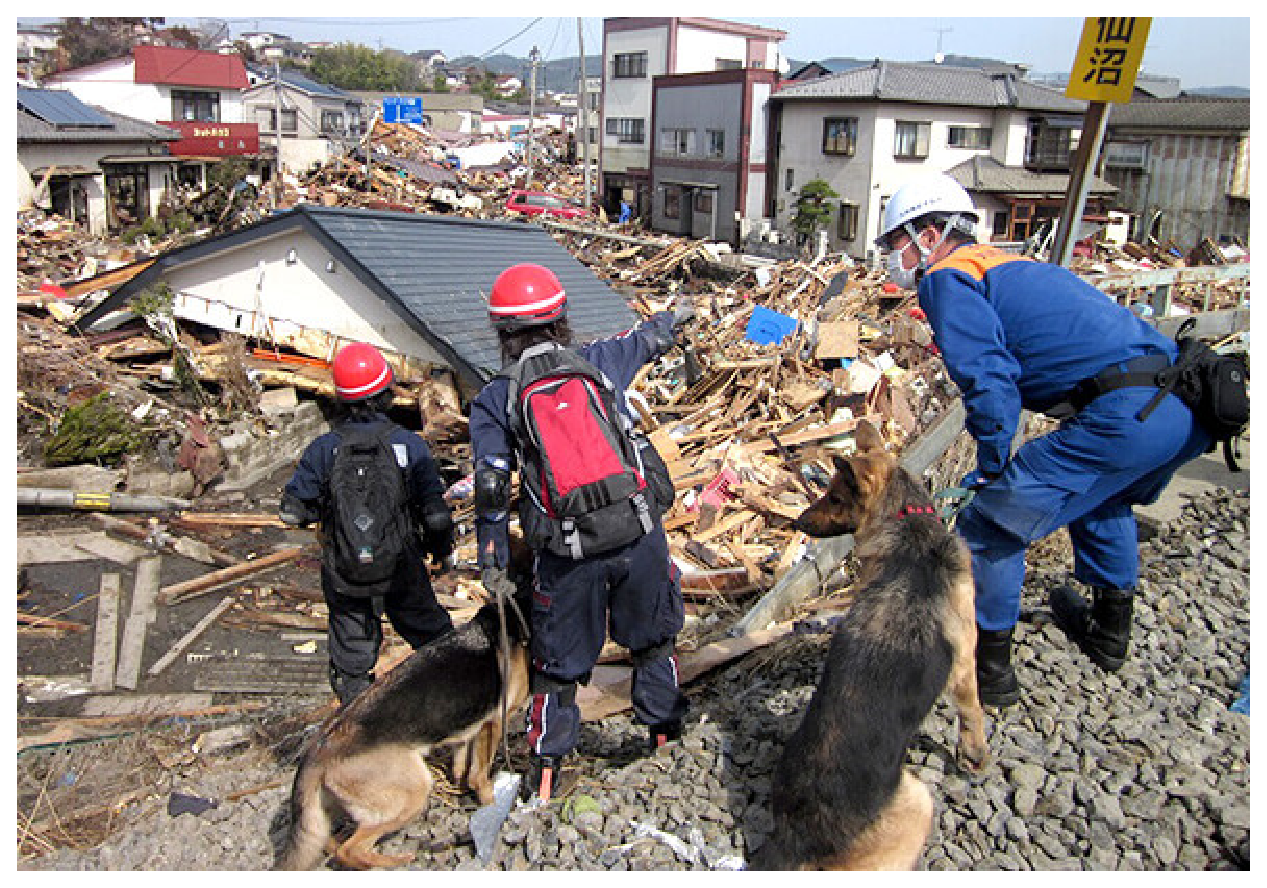
\includegraphics[width=6cm]{./Figures/resque.eps}
  \caption{被災地におけるレスキュー犬らの救助活動~\cite{buycott}より引用}
  \label{resque}
 \end{center}
\end{figure}
